\documentclass[12pt, a4paper]{article}
\usepackage{../../../myconfig} % Gọi file cấu hình từ ngoài gốc vào

% ==========================================
% BẮT ĐẦU NỘI DUNG TÀI LIỆU
% ==========================================
\begin{document}

% Truyền 3 tham số: {Nhãn cam} {Chữ to chính giữa} {Chữ ở góc phải Header}
\titlebox{Chủ đề: Tích phân}{Ứng dung tích phân tính diện tích thể tính}{Nguyên hàm - Tích phân: Ứng dụng}

\drawdashlines{27}
\newpage
\drawdashlines{33}
\newpage
\drawdashlines{33}
\newpage
\drawdashlines{33}
\newpage
\begin{figure}[htbp]
    
    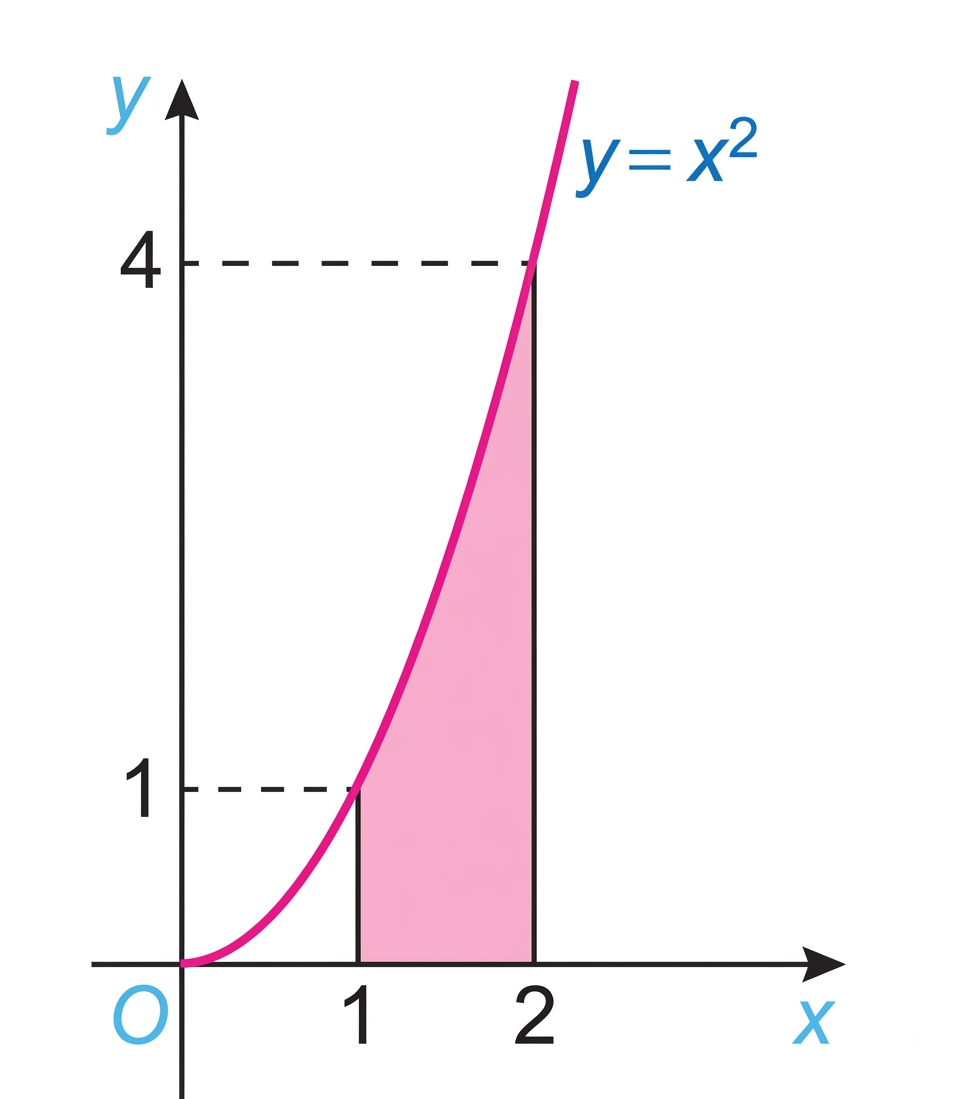
\includegraphics[width=0.4\textwidth]{images/H1.png}
    \quad
    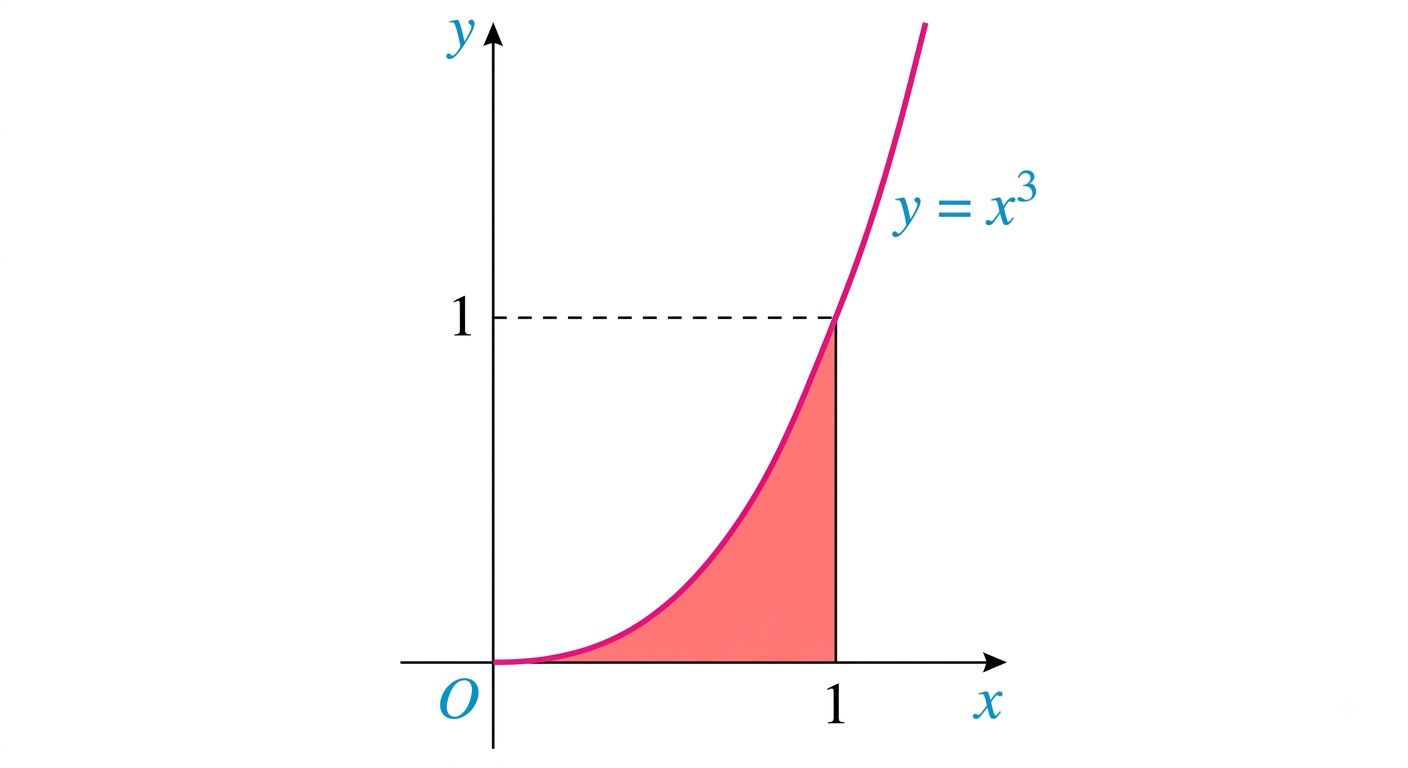
\includegraphics[width=0.8\textwidth]{images/H2.png}
\end{figure}
\drawdashlines{20}
\newpage
\begin{figure}[htbp]
    
    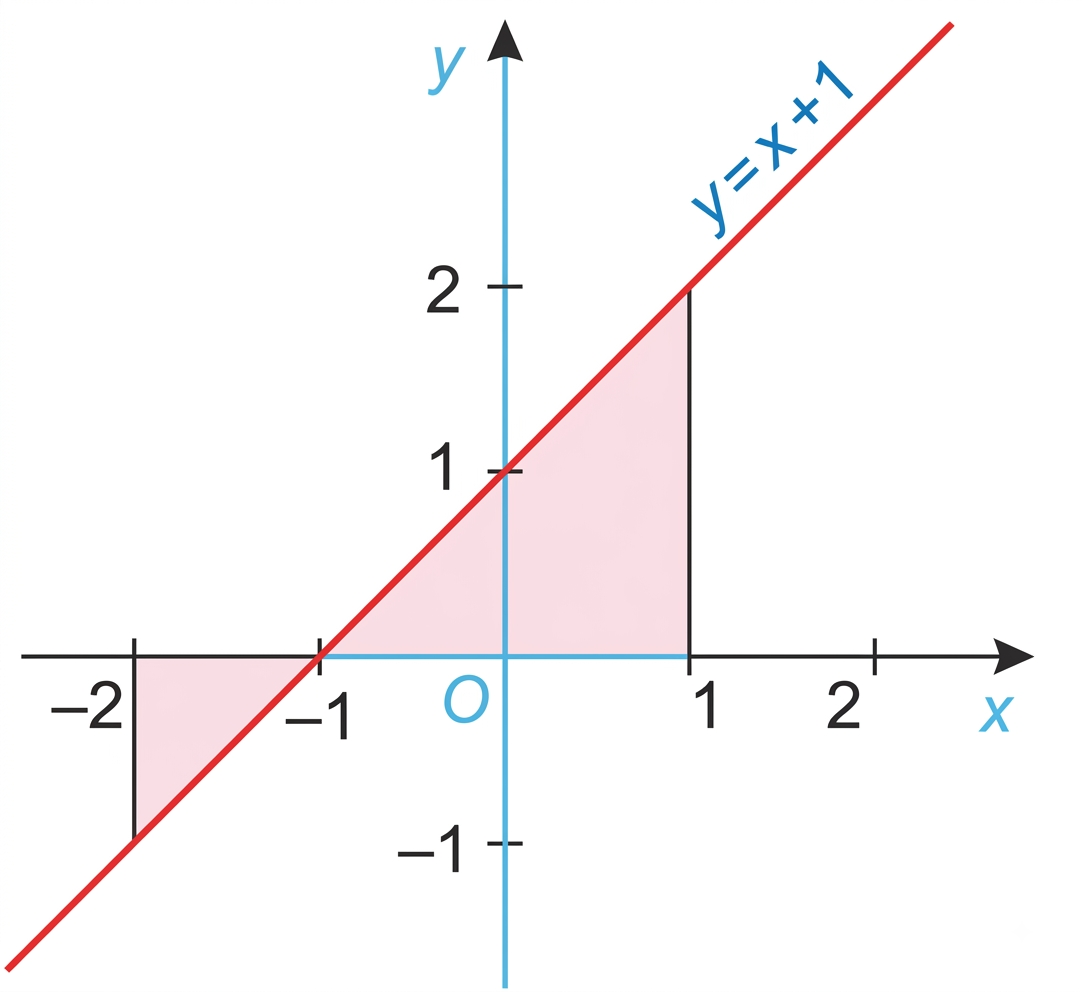
\includegraphics[width=0.4\textwidth]{images/H3.png}
\end{figure}
\drawdashlines{20}
\begin{figure}[htbp]
    
    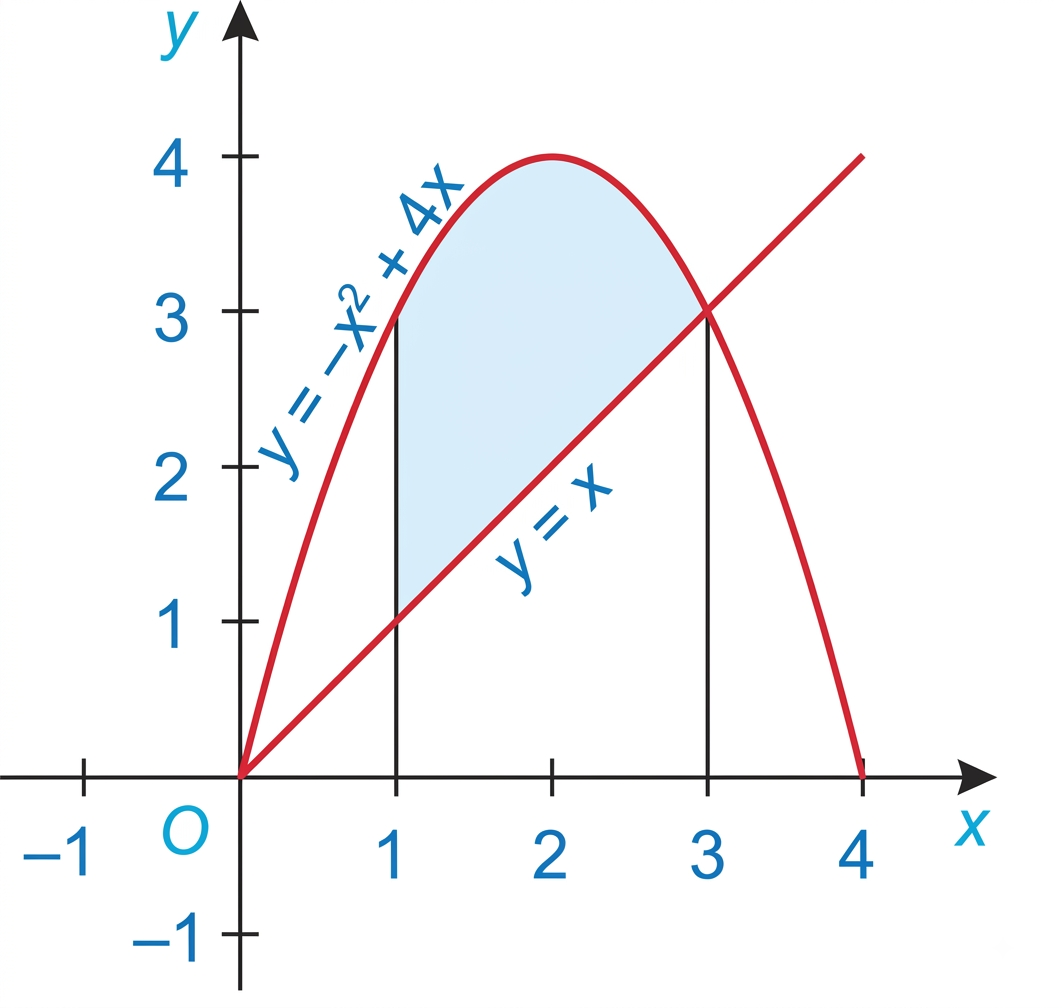
\includegraphics[width=0.4\textwidth]{images/H4.png}
\end{figure}
\drawdashlines{20}
\begin{figure}[htbp]
    
    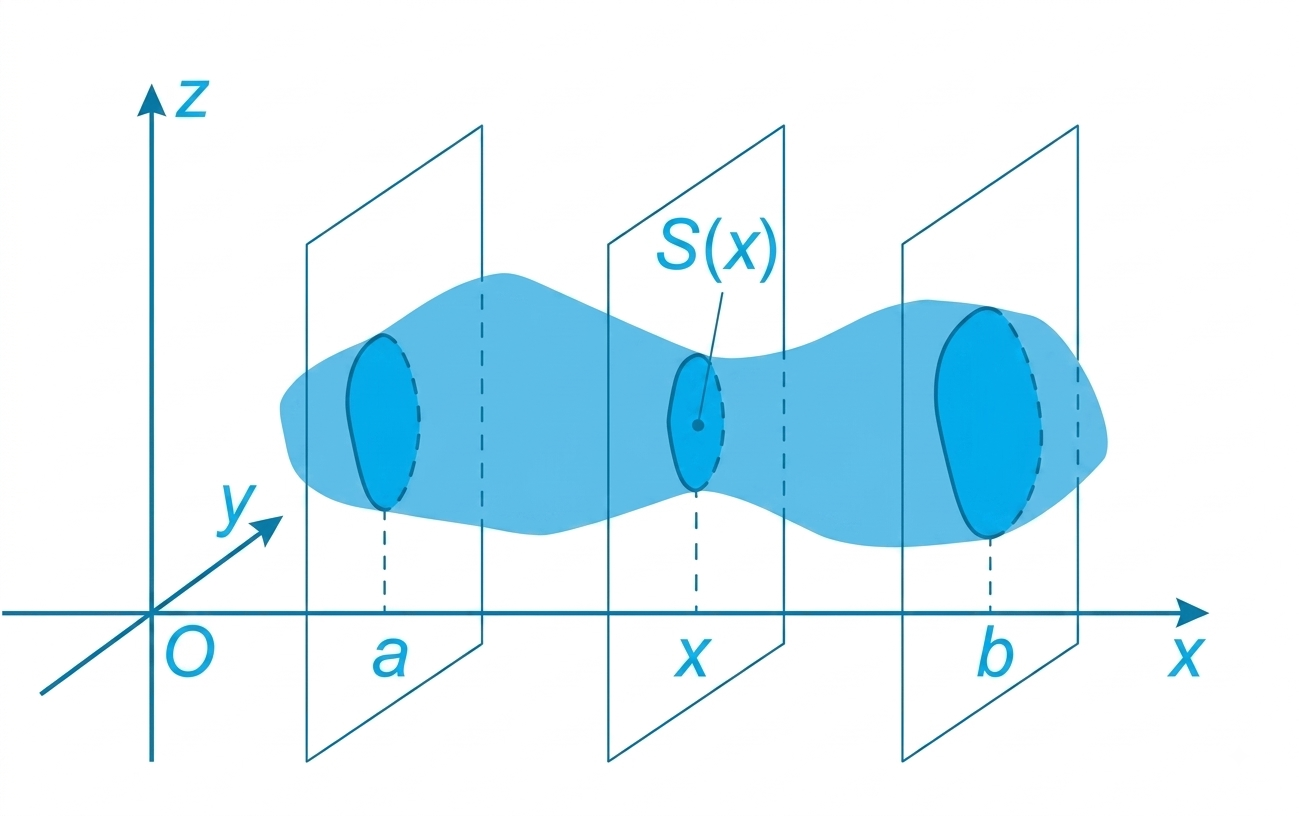
\includegraphics[width=0.5\textwidth]{images/H5.png}
\end{figure}
\drawdashlines{8}
\begin{figure}[htbp]
    
    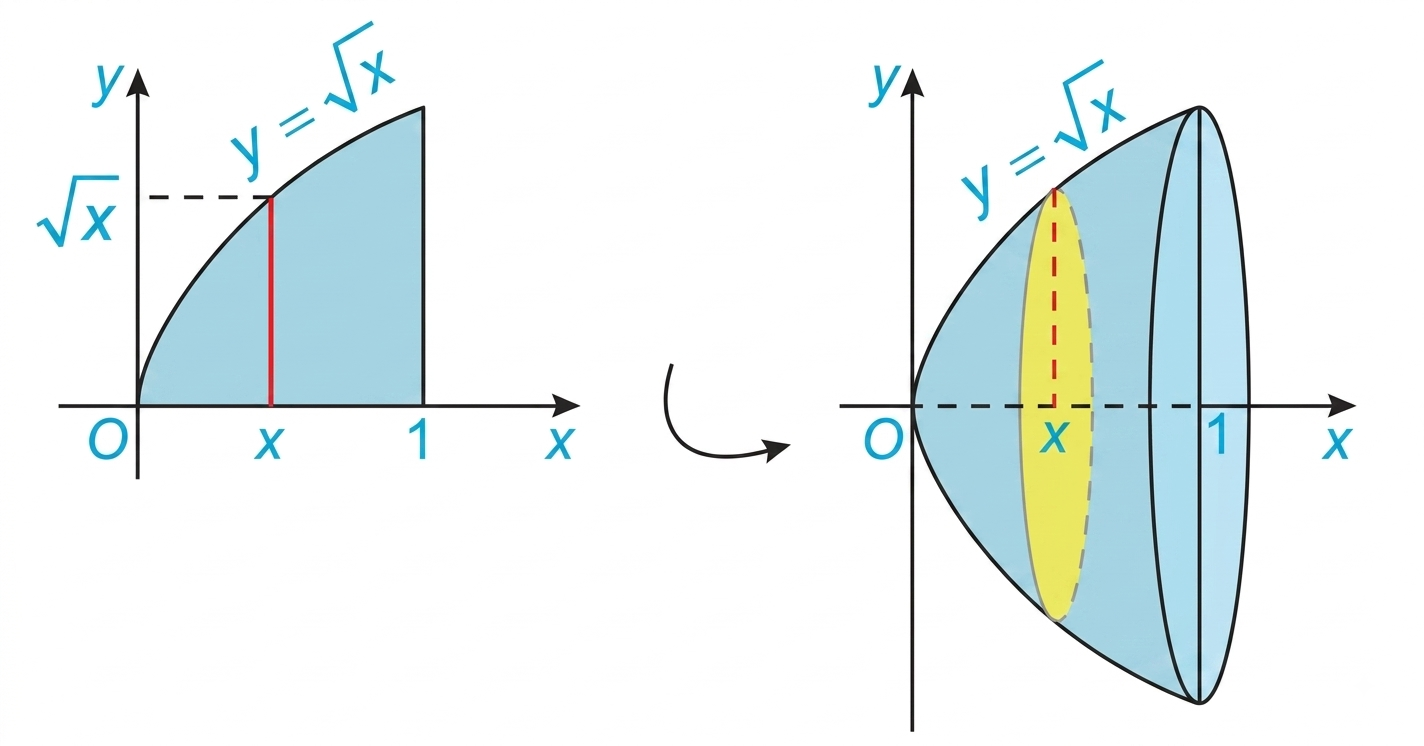
\includegraphics[width=0.5\textwidth]{images/H6.png}
\end{figure}
\drawdashlines{10}
\newpage
\drawdashlines{30}
\newpage

% --- CÂU 1 ---
\questionLinesManual{14}{1}{Trong mặt phẳng với hệ tọa độ \( Oxy \), diện tích \( S \) của hình phẳng giới hạn bởi đồ thị hàm số \( y = 2x + 1 \), trục hoành và hai đường thẳng \( x = 1, \, x = 2 \) được xác định bằng công thức}{%
    \begin{tasks}(4)
        \task \( S = \displaystyle\int_{1}^{2} (2x + 1)^2 dx. \)
        \task \( S = \displaystyle\pi \int_{1}^{2} (2x + 1)^2 dx. \)
        \task \( S = \displaystyle\int_{1}^{2} (2x + 1) dx. \)
        \task \( S = \displaystyle\int_{1}^{2} (-2x - 1) dx. \)
    \end{tasks}
}

% --- CÂU 2 ---
\questionLinesManual{14}{2}{Trong mặt phẳng với hệ tọa độ \( Oxy \), diện tích \( S \) của hình phẳng giới hạn bởi đồ thị của hàm số \( y = 2x - 3 \), trục hoành và hai đường thẳng \( x = 0, \, x = 1 \) được xác định bằng công thức}{%
    \begin{tasks}(4)
        \task \( S = \displaystyle\int_{0}^{1} (2x - 3) dx. \)
        \task \( S = \displaystyle\int_{0}^{1} (2x - 3) dx. \)
        \task \( S = \displaystyle\int_{0}^{1} (3-2x) dx. \)
        \task \( S = \displaystyle\pi \int_{0}^{1} (2x - 3)^2 dx. \)
    \end{tasks}
}

% --- CÂU 3 ---
\questionLinesManual{15}{3}{Diện tích phần gạch sọc trong hình vẽ bằng:

\begin{center}
\begin{tikzpicture}[>=latex, scale=0.8]
    % Thư viện cần dùng cho tô gạch chéo: \usetikzlibrary{patterns}
    
    % 1. Tô miền gạch chéo giữa đường thẳng và parabola từ x = -3 đến x = 1
    \fill[pattern=north east lines] 
        plot[domain=-3:1, samples=100] (\x, {-\x + 1}) -- 
        plot[domain=1:-3, samples=100] (\x, {\x*\x + \x - 2}) -- cycle;

    % 2. Trục tọa độ
    \draw[->] (-4,0) -- (3,0) node[above] {\small $x$};
    \draw[->] (0,-3) -- (0,5) node[right] {\small $y$};
    \node[below left] at (0,0) {\small $O$};

    % 3. Vẽ đồ thị
    % Parabola y = x^2 + x - 2
    \draw[thick, samples=100, domain=-3.2:2.2] 
        plot (\x, {\x*\x + \x - 2}) 
        node[below right] {\small $y = x^2 + x - 2$};
    
    % Đường thẳng y = -x + 1
    \draw[thick, samples=100, domain=-3.5:2.2] 
        plot (\x, {-\x + 1}) 
        node[right] {\small $y = -x + 1$};

    % 4. Đường gióng và các điểm giao
    \draw[dashed] (-3,0) -- (-3,4);
    
    \fill (-3,0) circle (1.5pt) node[below] {\small $-3$};
    \fill (1,0) circle (1.5pt) node[below right] {\small $1$};
\end{tikzpicture}
\end{center}
}{%
    \begin{tasks}(2)
        \task \( S = \displaystyle\int_{-3}^{1} (-x^2 - 2x - 3) dx. \)
        \task \( S = \displaystyle\int_{-3}^{1} (x^2 - 2x - 3) dx. \)
        \task \( S = \displaystyle\int_{-3}^{1} (x^2 + 2x - 3) dx. \)
        \task \( S = \displaystyle\int_{-3}^{1} (-x^2 - 2x + 3) dx. \)
    \end{tasks}
}

% --- CÂU 4 ---
\questionLinesManual{15}{4}{Diện tích phần hình phẳng gạch chéo trong hình vẽ bên được tính theo công thức nào dưới đây?

\begin{center}
\begin{tikzpicture}[>=latex, scale=1.0]
    % 1. Vẽ hệ trục tọa độ
    \draw[->, black, thick] (-2.5, 0) -- (3.5, 0) node[below] {\small $x$};
    \draw[->, black, thick] (0, -2.5) -- (0, 4.5) node[right] {\small $y$};
    \node[below left] at (0,0) {\small $O$};
    
    % 2. Vẽ đồ thị hai hàm số
    % y = x^2 - 2x - 1 (parabol quay lên)
    \draw[ultra thick, samples=150, domain=-1.5:3.5] 
        plot (\x, {\x*\x - 2*\x - 1});
        \node at (4.5,2) {$y = x^2 - 2x - 1$};
    
    % y = -x^2 + 3 (parabol quay xuống)
    \draw[ultra thick, samples=150, domain=-2.5:2.5] 
        plot (\x, {-\x*\x + 3});
        \node at (4,-2) {$y = -x^2 + 3$};
    
    % 3. Tô phần gạch chéo (phần giới hạn bởi hai đồ thị từ -1 đến 2)
    \fill[pattern=north east lines, pattern color=gray!50, domain=-1:2, variable=\x]
        plot (\x, {-\x*\x + 3}) -- plot (\x, {\x*\x - 2*\x - 1}) -- cycle;
    
    % 4. Đánh dấu các điểm đặc biệt
    % Giao điểm của hai đồ thị tại x = -1 và x = 2
    \draw[dashed, black] (-1,0) -- (-1,2) -- (0,2);
    \node[below] at (-1,0) {\small $-1$};
    \node[left] at (0,2) {\small $2$};
    \fill (-1,2) circle (2pt);
    
    \draw[dashed, black] (2,0) -- (2,-1) -- (0,-1);
    \node[below] at (2,0) {\small $2$};
    \node[left] at (0,-1) {\small $-1$};
    \fill (2,-1) circle (2pt);
    
    % Đỉnh của parabol y = -x^2 + 3 tại (0, 3)
    \draw[dashed, black] (0,3) -- (0,0);
    \node[left] at (0,3) {\small $3$};
    \fill[red] (0,3) circle (2pt);
    
    % Đỉnh của parabol y = x^2 - 2x - 1 tại (1, -2)
    \draw[dashed, black] (1,0) -- (1,-2) -- (0,-2);
    \node[below] at (1,0) {\small $1$};
    \node[left] at (0,-2) {\small $-2$};
    \fill[blue] (1,-2) circle (2pt);
    
\end{tikzpicture}
\end{center}
}{%
    \begin{tasks}(2)
        \task \( S = \displaystyle\int_{-1}^{2} (2x^2 - 2x - 4) dx. \)
        \task \( S = \displaystyle\int_{-1}^{2} (2x^2 + 2x - 4) dx. \)
        \task \( S = \displaystyle\int_{-1}^{2} (-2x^2 + 2x + 4) dx. \)
        \task \( S = \displaystyle\int_{-1}^{2} (-2x^2 - 2x + 4) dx. \)
    \end{tasks}
}

% --- CÂU 5 ---
\questionLinesManual{15}{5}{Diện tích hình phẳng được giới hạn bởi đồ thị hàm số \( y = f(x) \), trục hoành, trục tung và đường thẳng \( x = a \), \( a > 0 \) (phần tô đậm trong hình vẽ) được tính theo công thức

\begin{center}
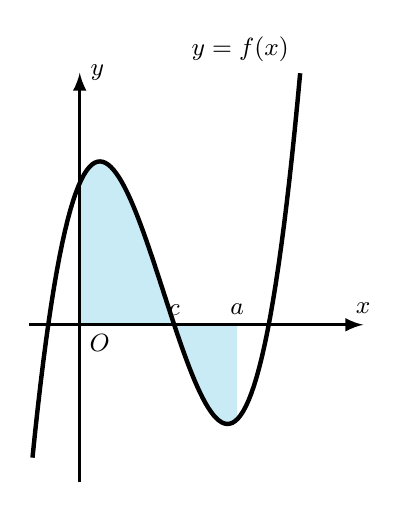
\begin{tikzpicture}[>=latex, scale=0.8]
    % Định nghĩa màu sắc xanh dương đậm giống trong hình
    \definecolor{darkblue}{RGB}{0, 0, 128}
    \definecolor{cyanfill}{RGB}{200, 235, 245}

    % 1. Tô màu phần diện tích
    % Miền trên trục hoành (từ x=0 đến x=2)
    \fill[cyanfill] 
        plot[domain=0:2.5, samples=100] (\x, {(\x+0.5) *(\x-1.5)*(\x-3)}) -- 
        (2.5,0) -- (0,0) -- cycle;

    

    % 2. Trục tọa độ
    \draw[->, very thick] (-0.8,0) -- (4.5,0) node[above] {\small $x$};
    \draw[->, very thick ] (0,-2.5) -- (0,4) node[right] {\small $y$};
    \node[below right] at (0,0) {\small $O$};

    % 3. Đồ thị hàm số y = f(x)
    \draw[ultra thick, samples=100, domain=-0.75:3.5] 
        plot (\x, {(\x+0.5) *(\x-1.5)*(\x-3)}) 
        node[above left] {\small $y = f(x)$};
    
    \node[above] at (1.5,0) {\small $c$};
    \node[above] at (2.5,0) {\small $a$};
\end{tikzpicture}
\end{center}
}{%
    \begin{tasks}(2)
        \task \( S = \displaystyle\int_{0}^{c} f(x) dx - \int_{a}^{c} f(x) dx. \)
        \task \( S = -\displaystyle\int_{0}^{a} f(x) dx. \)
        \task \( S = -\displaystyle\int_{0}^{c} f(x) dx + \int_{a}^{c} f(x) dx. \)
        \task \( S = \displaystyle\int_{0}^{c} f(x) dx + \int_{a}^{c} f(x) dx. \)
    \end{tasks}
}

% --- CÂU 6 ---
\questionLinesManual{15}{6}{Cho hàm số \( y = f(x) \) có đồ thị như hình sau và diện tích hai phần \( A, B \) lần lượt bằng 11 và 2. Khi đó giá trị của \( \int_{-2}^{1} f(x)dx \) bằng

\begin{center}
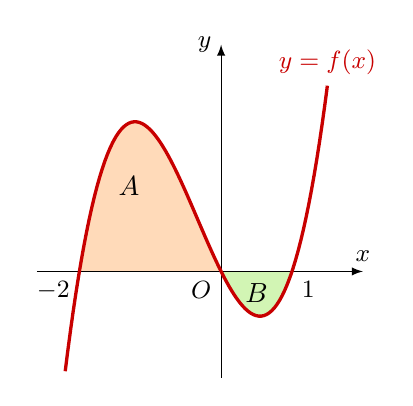
\begin{tikzpicture}[>=latex, scale=0.9]
    % Định nghĩa màu tô cho miền A và miền B
    \definecolor{colorA}{RGB}{255, 218, 185} % Màu cam nhạt
    \definecolor{colorB}{RGB}{210, 245, 180} % Màu xanh lá nhạt
    \definecolor{redline}{RGB}{200, 0, 0}    % Màu đỏ của đường cong

    % 1. Tô màu miền A (từ x = -2 đến x = 0)
    \fill[colorA] 
        plot[domain=-2:0, samples=100] (\x, {\x*(\x+2)*(\x-1)}) -- 
        (0,0) -- (-2,0) -- cycle;

    % 2. Tô màu miền B (từ x = 0 đến x = 1)
    \fill[colorB] 
        plot[domain=0:1, samples=100] (\x, {\x*(\x+2)*(\x-1)}) -- 
        (1,0) -- (0,0) -- cycle;

    % 3. Trục tọa độ
    \draw[->] (-2.6,0) -- (2.0,0) node[above] {\small $x$};
    \draw[->] (0,-1.5) -- (0,3.2) node[left] {\small $y$};
    \node[below left] at (0,0) {\small $O$};

    % 4. Đồ thị hàm số y = f(x)
    \draw[very thick, redline, samples=100, domain=-2.2:1.5] 
        plot (\x, {\x*(\x+2)*(\x-1)}) 
        node[above] {\small $y = f(x)$};

    % 5. Nhãn miền A, B và các mốc giá trị
    \node at (-1.3, 1.2) { $A$};
    \node at (0.5, -0.3) {$B$};

    \node[below left] at (-2,0) {\small $-2$};
    \node[below right] at (1,0) {\small $1$};
\end{tikzpicture}
\end{center}
}{%
    \begin{tasks}(4)
        \task 31
        \task 90
        \task 13
        \task 9
    \end{tasks}
}

% --- CÂU 7 ---
\questionLinesManual{12}{7}{Gọi \( S \) là diện tích hình phẳng giới hạn bởi đồ thị của hàm số  
\((H): y = \dfrac{x-1}{x+1}\)
và các trục tọa độ. Khi đó giá trị của \( S \) bằng
}{%
    \begin{tasks}(4)
        \task \( 2\ln 2 - 1 \)
        \task \( \ln 2 + 1 \)
        \task \( \ln 2 - 1 \)
        \task \( 2\ln 2 + 1 \)
    \end{tasks}
}

% --- CÂU 8 ---
\questionLinesManual{12}{8}{Diện tích hình phẳng giới hạn bởi đồ thị các hàm số  
\( y = -x^2 + 2x + 1, \, y = 2x^2 - 4x + 1 \) là}{%
    \begin{tasks}(4)
        \task 8
        \task 5
        \task 4
        \task 10
    \end{tasks}
}

% --- CÂU 9 ---
\questionLinesManual{12}{9}{Tính diện tích hình phẳng giới hạn bởi hai đồ thị  
\( y = x^2 + 2x, \, y = x + 2 \).}{%
    \begin{tasks}(4)
        \task \(\dfrac{7}{2}\)
        \task \(\dfrac{9}{2}\)
        \task \(\dfrac{5}{2}\)
        \task \(\dfrac{11}{2}\)
    \end{tasks}
}

% --- CÂU 10 ---
\questionLinesManual{12}{10}{Gọi \( D \) là hình phẳng giới hạn bởi các đường \( y = e^{4x}, y = 0, x = 0 \) và \( x = 1 \). Thể tích của khối tròn xoay tạo thành khi quay \( D \) quanh trục \( Ox \) bằng}{%
    \begin{tasks}(4)
        \task \( \displaystyle\int_{0}^{1} e^{4x} dx \)
        \task \( \displaystyle\pi\int_{0}^{1} e^{8x} dx \)
        \task \( \displaystyle\pi\int_{0}^{1} e^{4x} dx \)
        \task \( \displaystyle\int_{0}^{1} e^{8x} dx \)
    \end{tasks}
}

% --- CÂU 11 ---
\questionLinesManual{12}{11}{Tính thể tích V của phần vật thể giới hạn bởi hai mặt phẳng \( x = 1 \) và \( x = 3 \), biết rằng khi cắt vật thể bởi mặt phẳng vuông góc với trục \( Ox \) tại điểm có hoành độ \( x \) (\( 1 \leq x \leq 3 \)) thì được thiết diện là một hình chữ nhật có độ dài hai cạnh là \( 3x \) và \( \sqrt{3x^2 - 2} \).}{%
    \begin{tasks}(4)
        \task \( V = \dfrac{124}{3} \)
        \task \( V = (32 + 2\sqrt{15})\pi \)
        \task \( V = 32 + 2\sqrt{15} \)
        \task \( V = \dfrac{124\pi}{3} \)
    \end{tasks}
}

% --- CÂU 12 ---
\questionLinesManual{12}{12}{Tính thể tích của vật thể tạo nên khi quay quanh trục Ox hình phẳng \( D \) giới hạn bởi đồ thị \( (P): y = 2x - x^2 \) và trục Ox bằng:}{%
    \begin{tasks}(4)
        \task \( V = \dfrac{19\pi}{15} \)
        \task \( V = \dfrac{13\pi}{15} \)
        \task \( V = \dfrac{17\pi}{15} \)
        \task \( V = \dfrac{16\pi}{15} \)
    \end{tasks}
}

% --- CÂU 12 ---
\questionLinesManual{20}{13}{Tìm công thức tính thể tích của khối tròn xoay khi cho hình phẳng giới hạn bởi parabol  
\((P): y = x^2\) và đường thẳng \(d: y = 2x\) quay xung quanh trục \(Ox\).}{%
    \begin{tasks}(2)
        \task \( \displaystyle\pi\int_{0}^{2} (x^2 - 2x)^2 dx \)
        \task \( \displaystyle\pi\int_{0}^{2} 4x^2 dx - \pi\int_{0}^{2} x^4 dx \)
        \task \( \displaystyle\pi\int_{0}^{2} 4x^2 dx + \pi\int_{0}^{2} x^4 dx \)
        \task \( \displaystyle\pi\int_{0}^{2} (2x - x^2) dx \)
    \end{tasks}
}

% --- CÂU 14 ---
\questionLinesManual{20}{14}{Tính diện tích phần hình phẳng gạch chéo (tam giác cong OAB) trong hình vẽ bên.

\begin{center}
\begin{tikzpicture}[>=latex, scale=0.9]
    % Thư viện cần dùng: \usetikzlibrary{patterns}

    % 1. Tô miền gạch chéo
    % Miền từ x = 0 đến x = 1 (dưới đường y = x)
    \fill[pattern=north east lines] 
        (0,0) -- (1,1) -- (1,0) -- cycle;
        
    % Miền từ x = 1 đến x = 2 (dưới đường y = (x-2)^2)
    \fill[pattern=north east lines] 
        plot[domain=1:2, samples=100] (\x, {(\x - 2)^2}) -- 
        (2,0) -- (1,0) -- cycle;

    % 2. Lưới ô vuông nhạt
    \draw[gray!30, very thin] (-1.5,-1.5) grid (4.5,3.5);

    % 3. Trục tọa độ
    \draw[->, thick] (-1.5,0) -- (4.5,0) node[above] {\small $x$};
    \draw[->, thick] (0,-1.5) -- (0,3.5) node[right] {\small $y$};
    \node[below left] at (0,0) {\small $O$};

    % 4. Đồ thị hàm số
    % Parabola y = (x - 2)^2
    \draw[very thick, samples=100, domain=0.2:3.8] 
        plot (\x, {(\x - 2)^2}) 
        node[right] {\small $y = (x-2)^2$};

    % Đường thẳng y = x
    \draw[thick, gray!80, domain=-1.2:3.2] 
        plot (\x, {\x}) 
        node[above left] {\small $y = x$};

    % 5. Đường gióng nét đứt và các điểm
    \draw[dashed] (0,1) -- (1,1) -- (1,0);

    \fill (1,1) circle (1.5pt) node[right] {\small $A$};
    \fill (2,0) circle (1.5pt) node[above] {\small $B$};

    \node[below] at (1,0) {\small $1$};
    \node[below] at (2,0) {\small $2$};
    \node[left] at (0,1) {\small $1$};
    \node[left] at (0,2) {\small $2$};
\end{tikzpicture}
\end{center}
}{%
    \begin{tasks}(4)
        \task \( \dfrac{5}{6} \)
        \task \( \dfrac{5\pi}{6} \)
        \task \( \dfrac{8}{15} \)
        \task \( \dfrac{8\pi}{15} \)
    \end{tasks}
}

% --- CÂU 15 ---
\questionLinesManual{20}{15}{Cho \((H)\) là hình phẳng giới hạn bởi các đường \(y = \sqrt{x}\), \(y = x - 2\) và trục hoành. Diện tích của \((H)\) bằng

\begin{center}
\begin{tikzpicture}[>=latex, scale=0.9]
    % Thư viện cần dùng: \usetikzlibrary{patterns}

    % 1. Tô miền gạch chéo
    % Miền từ x = 0 đến x = 2 (dưới đường y = sqrt(x))
    \fill[pattern=north east lines] 
        plot[domain=0:2, samples=100] (\x, {sqrt(\x)}) -- 
        (2,0) -- (0,0) -- cycle;
        
    % Miền từ x = 2 đến x = 4 (giữa y = sqrt(x) và y = x - 2)
    \fill[pattern=north east lines] 
        plot[domain=2:4, samples=100] (\x, {sqrt(\x)}) -- 
        plot[domain=4:2, samples=100] (\x, {\x - 2}) -- cycle;

    % 2. Trục tọa độ
    \draw[->, thick] (-0.8,0) -- (5.2,0) node[below] {\small $x$};
    \draw[->, thick] (0,-0.8) -- (0,2.8) node[left] {\small $y$};
    \node[below left] at (0,0) {\small $O$};

    % 3. Đồ thị các hàm số
    % Đường cong y = sqrt(x)
    \draw[thick, samples=100, domain=0:5] 
        plot (\x, {sqrt(\x)})
        node[above] at (1,1.3) {\small $y = \sqrt{x}$};

    % Đường thẳng y = x - 2 (đi qua (2,0) và (4,2))
    \draw[thick, domain=1.2:4.6] 
        plot (\x, {\x - 2});

    % 4. Đường gióng nét đứt và điểm mốc
    \draw[dotted, thick] (0,2) -- (4,2) -- (4,0);

    \node[below] at (2,0) {\small $2$};
    \node[below] at (4,0) {\small $4$};
    \node[left] at (0,2) {\small $2$};
\end{tikzpicture}
\end{center}
}{%
    \begin{tasks}(4)
        \task \(\dfrac{7}{3}\)
        \task \(\dfrac{8}{3}\)
        \task \(\dfrac{10}{3}\)
        \task \(\dfrac{16}{3}\)
    \end{tasks}
}

% --- CÂU 16 ---
\questionLinesManual{20}{16}{Tính thể tích của vật thể tròn xoay thu được khi quay hình phẳng trong hình (phần được tô đậm) quanh trục Ox.
\begin{center}
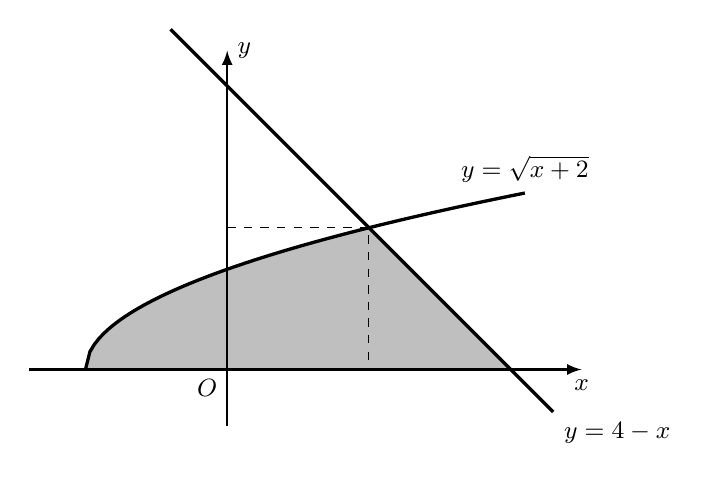
\begin{tikzpicture}[>=latex, scale=0.9]
    % 1. Tô màu xám miền giới hạn
    % Miền từ x = -2 đến x = 2 (dưới đường y = sqrt(x+2))
    \fill[gray!50] 
        plot[domain=-2:2, samples=100] (\x, {sqrt(\x + 2)}) -- 
        (2,0) -- (-2,0) -- cycle;
        
    % Miền từ x = 2 đến x = 4 (dưới đường y = 4 - x)
    \fill[gray!50] 
        (2,0) -- (2,2) -- (4,0) -- cycle;

    % 2. Trục tọa độ
    \draw[->, thick] (-2.8,0) -- (5,0) node[below] {\small $x$};
    \draw[->, thick] (0,-0.8) -- (0,4.5) node[right] {\small $y$};
    \node[below left] at (0,0) {\small $O$};

    % 3. Đồ thị các hàm số
    % Đường cong y = sqrt(x + 2)
    \draw[very thick, samples=100, domain=-2:4.2] 
        plot (\x, {sqrt(\x + 2)}) 
        node[above] {\small $y = \sqrt{x+2}$};

    % Đường thẳng y = 4 - x
    \draw[very thick, domain=-0.8:4.6] 
        plot (\x, {4 - \x}) 
        node[below right] {\small $y = 4 - x$};

    % 4. Đường gióng nét đứt tại giao điểm (2,2)
    \draw[dashed] (0,2) -- (2,2) -- (2,0);
\end{tikzpicture}
\end{center}
}{%
    \begin{tasks}(4)
        \task \(\dfrac{31\pi}{3}\)
        \task \(\dfrac{32\pi}{3}\)
        \task \(\dfrac{34\pi}{3}\)
        \task \(\dfrac{35\pi}{3}\)
    \end{tasks}
}

% --- CÂU 17 ---
\questionLinesManual{20}{17}{Một người thợ mộc phác thảo đồ thị của các hàm số \( y = \sqrt{x} \) và \( y = \dfrac{x}{2} \) lên một mảnh gỗ, rồi cắt lấy phần diện tích nằm giữa hai đồ thị để làm thành vật trang trí (xem hình bên dưới, đơn vị trên mỗi trục tọa độ được tính bằng cm). Tính diện tích bề mặt gỗ bị cắt ra (đơn vị: \( cm^2 \), làm tròn kết quả đến hàng phần trăm).

\begin{center}
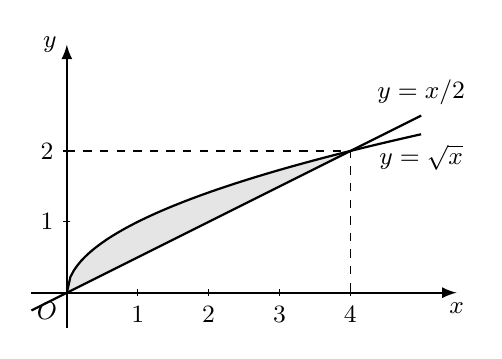
\begin{tikzpicture}[>=latex, scale=0.9]
    % 1. Tô màu phần diện tích giữa hai đồ thị
    \fill[gray!20] 
        plot[domain=0:4, samples=100] (\x, {sqrt(\x)}) -- 
        plot[domain=4:0, samples=100] (\x, {\x/2}) -- cycle;

    % 2. Trục tọa độ
    \draw[->, thick] (-0.5,0) -- (5.5,0) node[below] {\small $x$};
    \draw[->, thick] (0,-0.5) -- (0,3.5) node[left] {\small $y$};
    \node[below left] at (0,0) {\small $O$};

    % 3. Đánh dấu các mốc trên trục
    \foreach \x in {1,2,3,4} {
        \draw (\x,0.05) -- (\x,-0.05) node[below] {\small $\x$};
    }
    \draw (0.05,1) -- (-0.05,1) node[left] {\small $1$};
    \draw (0.05,2) -- (-0.05,2) node[left] {\small $2$};

    % 4. Đồ thị hàm số
    % Đường cong y = sqrt(x)
    \draw[thick, samples=100, domain=0:5] 
        plot (\x, {sqrt(\x)}) 
        node[below ] {\small $y = \sqrt{x}$};

    % Đường thẳng y = x/2
    \draw[thick, domain=-0.5:5] 
        plot (\x, {\x/2}) 
        node[above] {\small $y = x/2$};

    % 5. Đường gióng nét đứt
    \draw[dashed] (0,2) -- (4,2) -- (4,0);
\end{tikzpicture}
\end{center}
}

% --- CÂU 18 ---
\questionLinesManual{20}{18}{Cho một viên gạch men có dạng hình vuông \( OABC \) đã được gắn vào hệ trục tọa độ \( Oxy \) như hình bên dưới, với đơn vị trên mỗi trục tọa độ là \( dm \). Biết rằng hai đường cong của viên gạch ứng với các đồ thị hàm số \( y = x^3 \) và \( y = \sqrt{x} \). Diện tích phần họa tiết không được tô đậm của viên gạch (phần bên ngoài hình cong) bằng bao nhiêu \( cm^2 \)?

\begin{center}
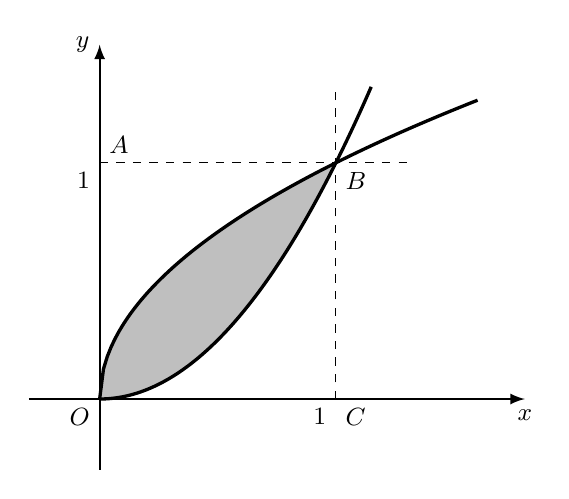
\begin{tikzpicture}[>=latex, scale=3]
    % 1. Tô màu xám miền giới hạn bởi y = sqrt(x) và y = x^2
    \fill[gray!50] 
        plot[domain=0:1, samples=100] (\x, {sqrt(\x)}) -- 
        plot[domain=1:0, samples=100] (\x, {\x*\x}) -- cycle;

    % 2. Trục tọa độ
    \draw[->, thick] (-0.3,0) -- (1.8,0) node[below] {\small $x$};
    \draw[->, thick] (0,-0.3) -- (0,1.5) node[left] {\small $y$};
    \node[below left] at (0,0) {\small $O$};

    % 3. Đồ thị các hàm số
    % Đường cong y = sqrt(x)
    \draw[very thick, samples=100, domain=0:1.6] 
        plot (\x, {sqrt(\x)});

    % Đường cong y = x^2
    \draw[very thick, samples=100, domain=0:1.15] 
        plot (\x, {\x*\x});

    % 4. Đường gióng nét đứt và các điểm A, B, C
    \draw[dashed] (0,1) -- (1.3,1);
    \draw[dashed] (1,0) -- (1,1.3);

    % Nhãn các điểm và mốc giá trị
    \node[below left] at (0,1) {\small $1$};
    \node[above right] at (0,1) {\small $A$};
    
    \node[below right] at (1,1) {\small $B$};
    
    \node[below left] at (1,0) {\small $1$};
    \node[below right] at (1,0) {\small $C$};
\end{tikzpicture}
\end{center}
}

\end{document}
